%# -*- coding: utf-8-unix -*-
%%==================================================
\chapter{文字检测(Scene Text Detection)}
近期的文字检测算法主要是解决曲形文本的检测问题。MATI\cite{li2019learning}和TextTubes\cite{seytre2019texttubes}都是通过直接预测文本的边界来描述曲形文本。
不同之处在于MATI是直接在全图预测边界点(single stage),而TextTubes\cite{seytre2019texttubes}是在MaskRCNN的基础上将mask head换为预测文本的属性来描述曲形文本。

DB\cite{liao2019real}是基于分割的方法,意在解决文本检测的效率问题。

随后,RelaText\cite{ma2020relatext},PuzzleNet\cite{liu2020puzzlenet}以及DRRG\cite{zhang2020deep}都是自下而上的方法:都是首先预测文本的组件,然后通过GCN
来预测文本组件之间的连接关系来完成检测任务。这些基于图卷积的方法不同之处在于graph的构建方式不同。
\section{文字检测方法介绍}
\subsection{MATI}
MATI\cite{li2019learning}主要是解决任意形状文本检测的问题。现有能够检测曲形文本的检测器大都是基于分割的方法,
如Textfield\cite{xu2019textfield}、TextSnake\cite{long2018textsnake}、CRAFT\cite{baek2019character}、PSENet\cite{wang2019shape}以及MaskRCNN\cite{he2017mask}。
但是基于分割方法往往需要预测文本区域的几何属性,结合复杂的后处理过程得到任意形状的文本区域,使得检测器后处理不够高效。
基于anchor box回归的方法虽然简单高效,但是任意形状文本难以使用包围盒进行描述。基于此,文章中提出使用直接回归的方法来检测任意形状文本。

\subsubsection{MATI的网络结构}
MATI的网络结构如图\ref{mati_framework}所示:网络的整体结构基于SSD,不同的是该方法中不需要anchor box,整体和east一样进行密集预测。
\begin{figure}[H]
    \centering
    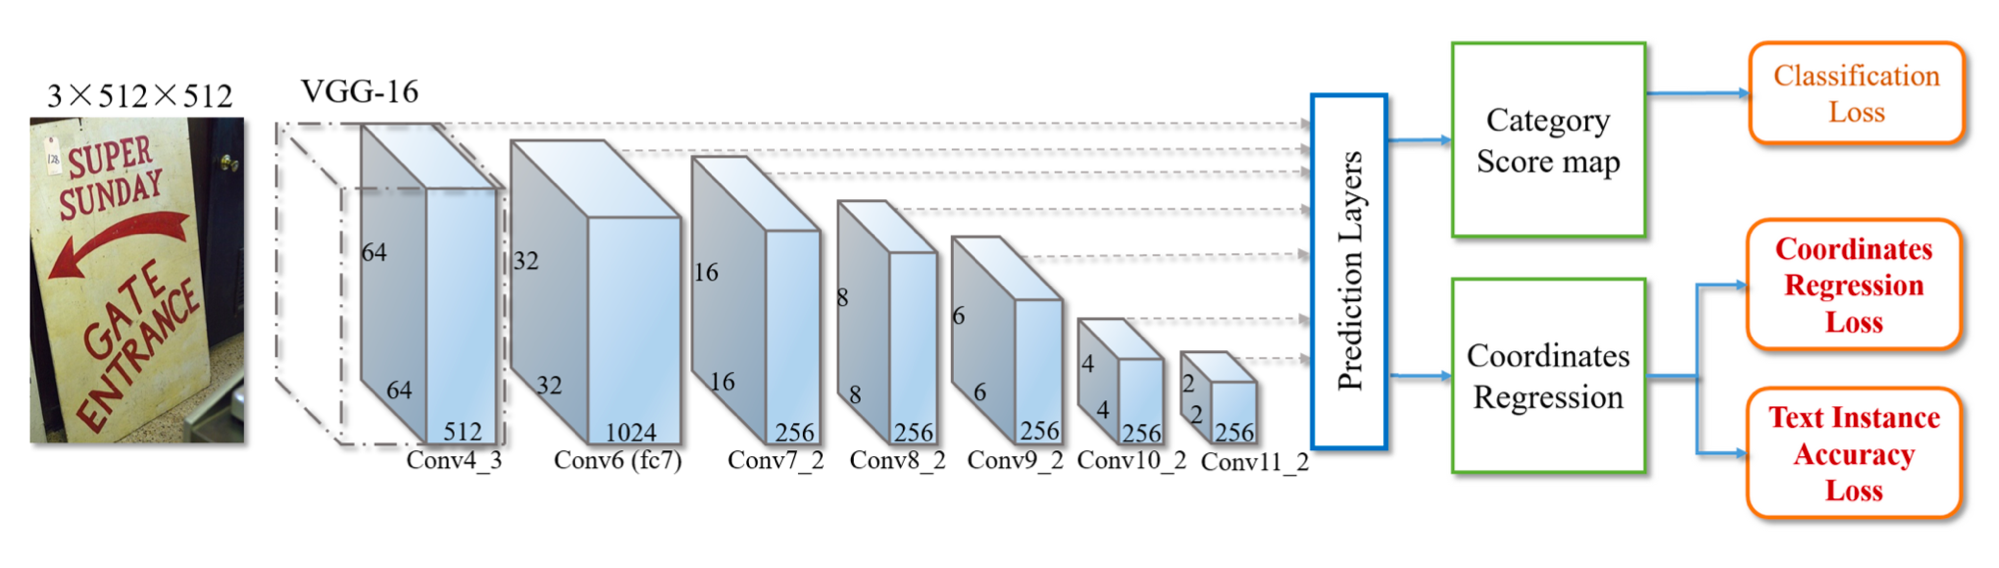
\includegraphics[width=.98\textwidth]{figure/detection/mati_framework.png} 
    \caption{MATI网络框架图。} 
    \label{mati_framework} 
\end{figure}

MATI的主要贡献在于:为了使得回归学得准确,提出Starting-point-independent Coordinates Regression Loss和Text Instance Accuracy Loss。
Starting-point-independent Coordinates Regression Loss如下:

$L_{reg} = \sum\limits_{m\in L_{reg}^{+}} \mathop{min}\limits_{j \in [0,...,n-1]} \sum\limits_{i=0}^{n-1} smooth_{L_{1}} (\hat{z}_{i}^{m} - z_{(j+i)\%n}^{m*})$,

其中$\hat{z}_{i}^{m}$是第m个文本实例的第i个预测顶点,$z_{i}^{m*}$是第m个文本实例的第i个顶点标注。该Loss的物理含义是:只需要计算预测点和标注中相邻最近的点的loss。

Text Instance Accuracy Loss如图\ref{mati_textrender}所示:将预测的点转化为mask和mask的gt之间计算IOU,具体如何将预测的点转化为mask没有具体说明,需查看对于参考文献。
\begin{figure}[H]
    \centering
    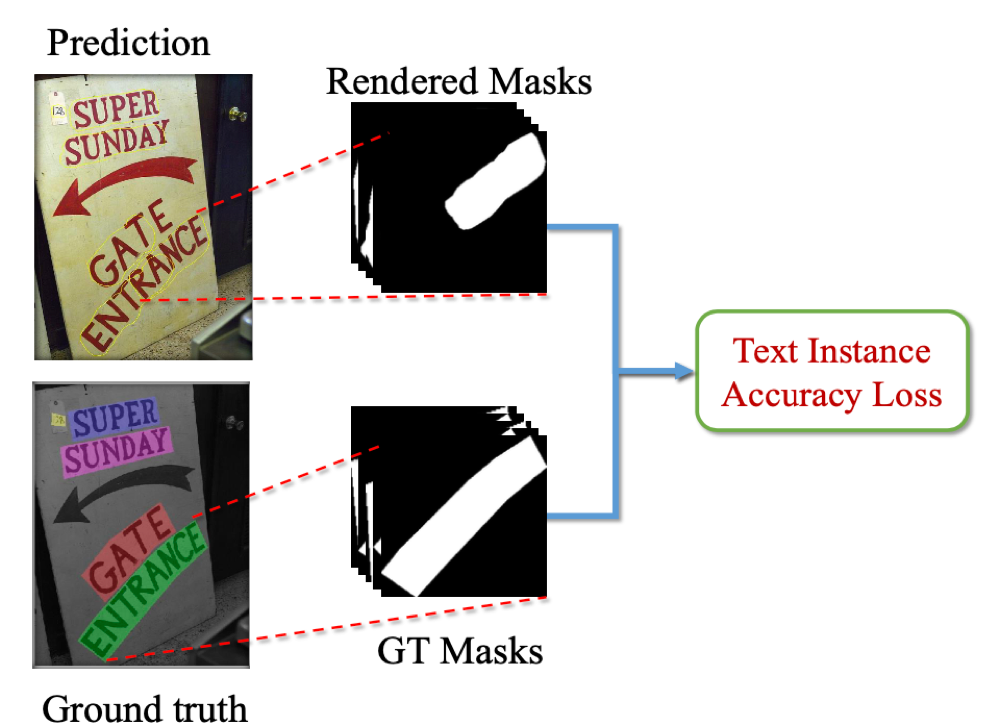
\includegraphics[width=.7\textwidth]{figure/detection/mati_textrender.png} 
    \caption{Text Instance Accuracy Loss。} 
    \label{mati_textrender} 
\end{figure}

\subsection{TextTubes}
TextTubes\cite{seytre2019texttubes}同样是针对曲形文本检测的问题,方法上属于基于回归的方法。该方法并不直接回归文本的边界点,而是通过回归出文本的中心轴,以及中心轴上垂直方法的半径来描述文本区域。

\subsubsection{TextTubes的网络结构}
TextTubes的网络结构如图\ref{texttubes_framework}所示:网络的整体结构基于MaskRCNN,将MaskRCNN的mask head更改为该方法中的Tube head(回归文本中心轴以及半径)。
\begin{figure}[H]
    \centering
    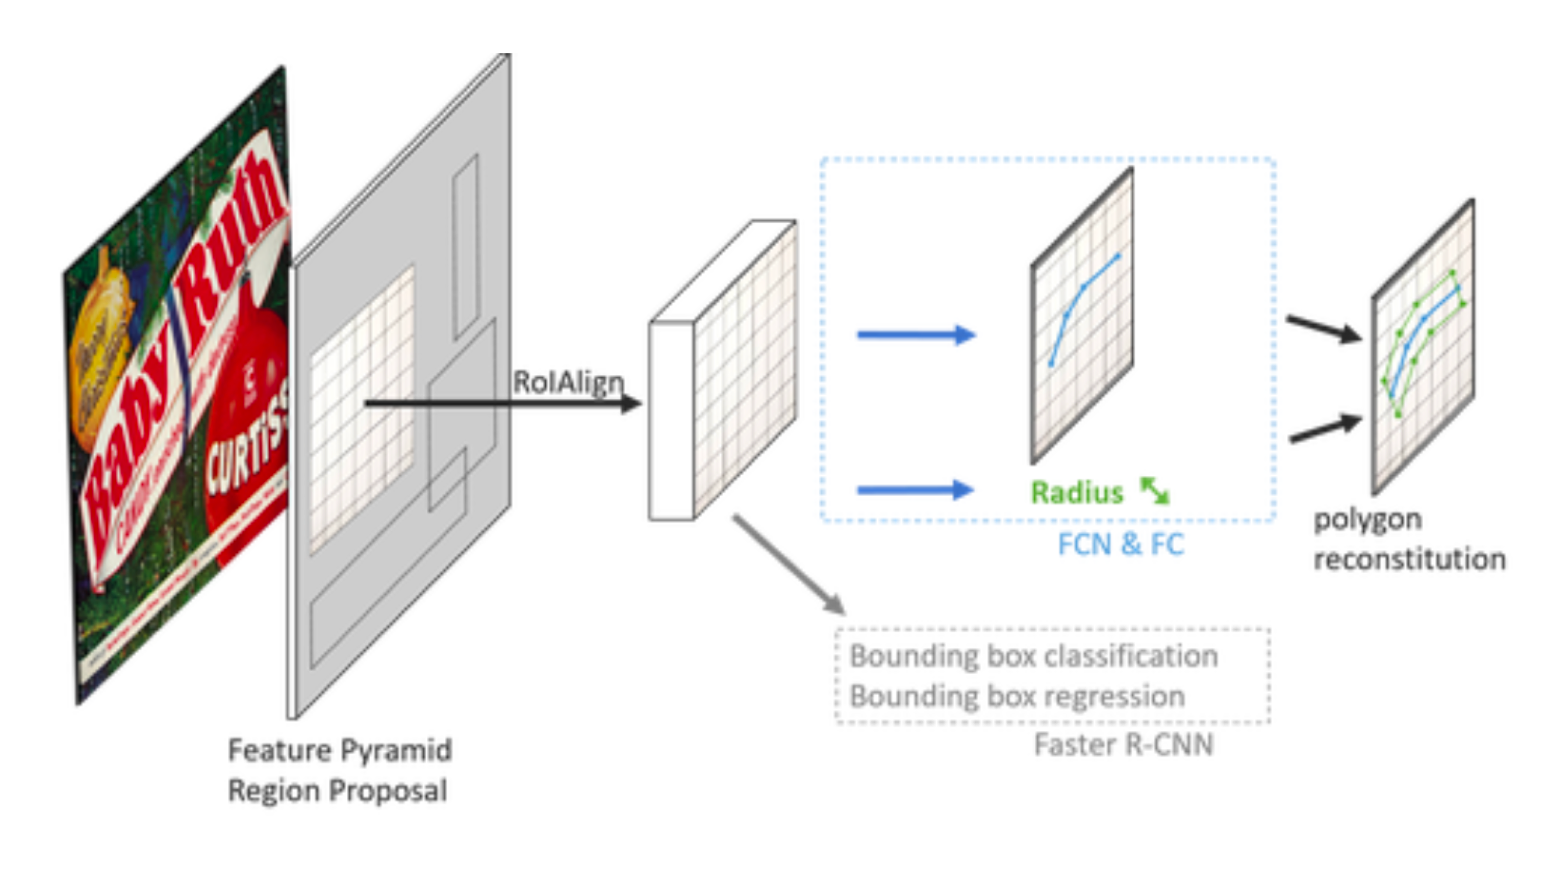
\includegraphics[width=.8\textwidth]{figure/detection/texttubes_framework.png} 
    \caption{TextTubes网络框架图。} 
    \label{texttubes_framework} 
\end{figure}

文中指出:文本的中心轴在训练时难以确定(中心轴附近的点也可算为中心轴区域),因此提出新的损失函数而不是直接进行回归中心轴上的点。新的损失函数定义如下:

$l_{tube} = l_{radius} + l_{axis} + l_{endpoints} + l_{spread}$

其中$l_{axis}$定义如下,其中$\hat{S}$表示回归的中心线的点的集合(回归4个点,采样100个点计算loss),

$l_{axis}(\hat{S},S) = 1 - \alpha\vartheta_{abs}(\hat{\gamma}, \gamma) - (1 - \alpha)\vartheta_{tan}(\hat{\gamma}, \gamma)$,

$\vartheta_{abs}(\hat{\gamma}, \gamma) = \int_{0}^{1}exp(-\frac{d(\hat{\gamma}(t) - \gamma(t))^{2}}{2\sigma^{2}})dt$, 
$\vartheta_{tan}(\hat{\gamma}, \gamma) = \int_{0}^{1}exp(-\frac{sin^{2}(\hat{\theta}(t) - \theta(t))}{2\sigma^{2}})dt$

$l_{axis}$的物理含义是:通过积分来计算预测的中心轴区域与gt的loss,使得整体上能够对齐。$\hat{\gamma}$的定义没有看的很明白,具体请参考原文。

\subsection{DB (AAAI2020)}
DB\cite{liao2019real}是基于分割的快速文本检测器。其快速的原因在于通过动态学习分割的阈值从而简化了分割图到contours的后处理过程。

\subsubsection{DB的网络结构}
DB的网络结构如图\ref{db_framework}所示:网络通过预测文本实例的分割图以及阈值图,然后通过比较分割图和阈值图得到二进制图(约化的二进制图)。
\begin{figure}[H]
    \centering
    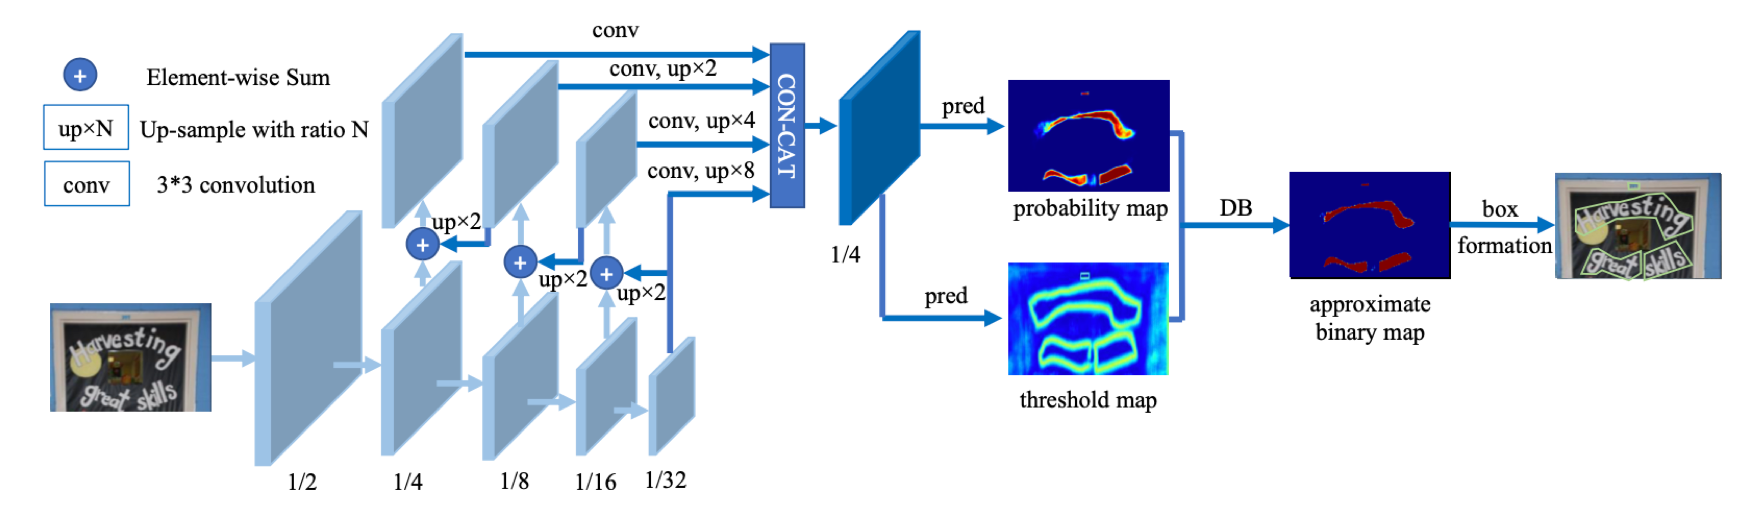
\includegraphics[width=.98\textwidth]{figure/detection/db_framework.png} 
    \caption{DB网络框架图。} 
    \label{db_framework} 
\end{figure}

DB的二值化函数如下:

$\hat{B}_{i,j} = \frac{1}{1 + e^{-k(P_{i,j} - T_{i,j})}}$,其中$P_{i,j}$代表分割图,其中$T_{i,j}$代表阈值图。
训练过程中,分割图和阈值图的ground truth如图\ref{db_gt}所示。
\begin{figure}[H]
    \centering
    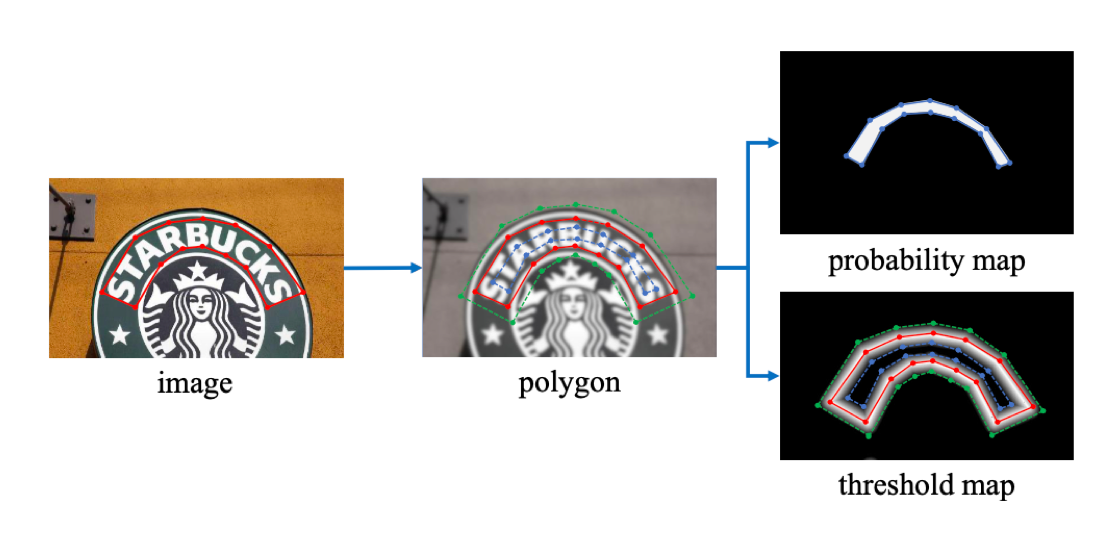
\includegraphics[width=.8\textwidth]{figure/detection/db_gt.png} 
    \caption{DB label制作过程。} 
    \label{db_gt} 
\end{figure}

\subsection{RelaText}
RelaText\cite{ma2020relatext}属于bottom-up类型的任意形状文本检测器。

\subsubsection{RelaText的网络结构}
RelaText的网络结构如图\ref{relatext_framework}所示:网络的整体结构基于FPN,采用Anchor-Free RPN\cite{zhong2019anchor}的架构。网络首先预测出文本的组件(由四边形构成,如图\ref{relatext_gt}所示),
然后将经过nms后保留的每个graph经过GCN来获得最终的文本实例区域。
\begin{figure}[H]
    \centering
    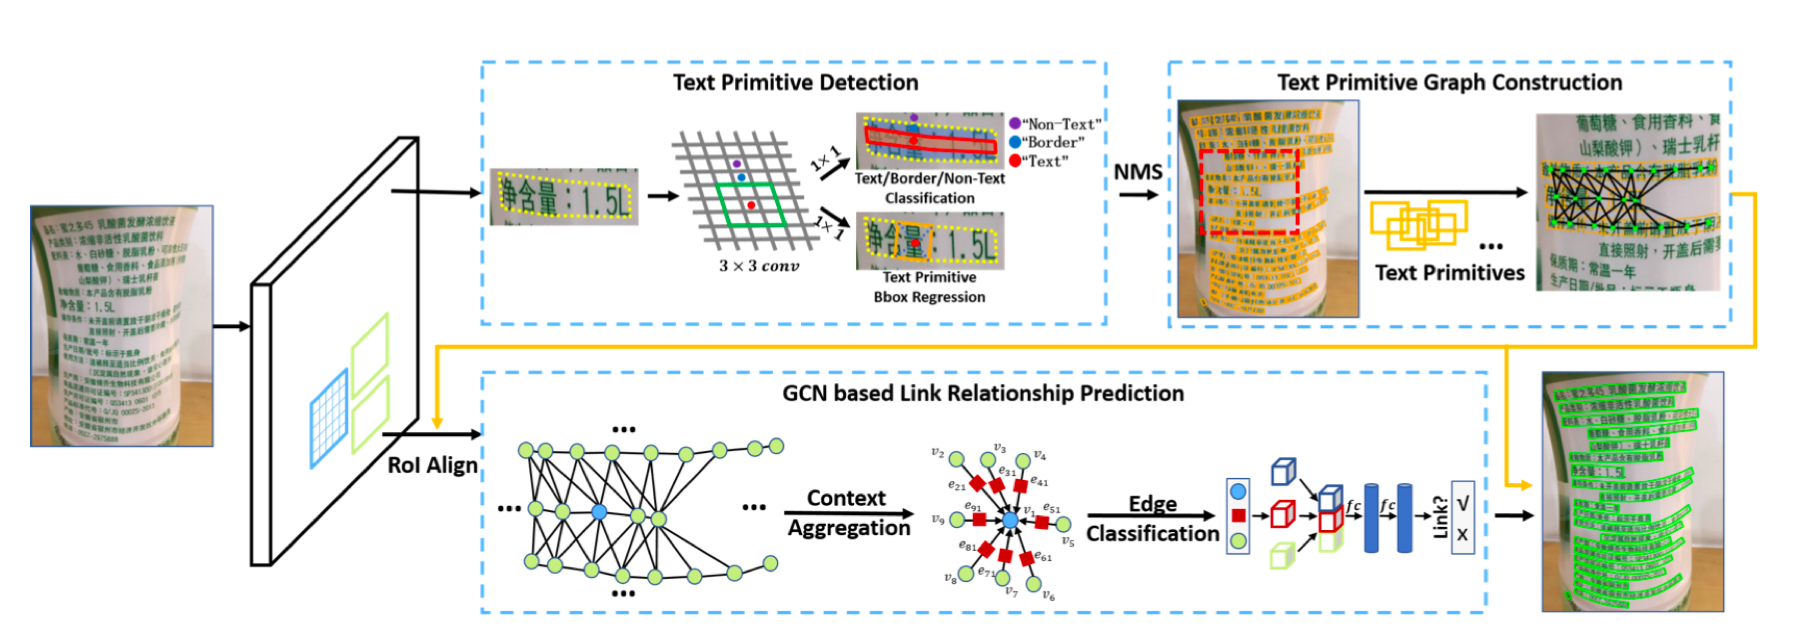
\includegraphics[width=.98\textwidth]{figure/detection/relatext_framework.png} 
    \caption{RelaText网络框架图。} 
    \label{relatext_framework} 
\end{figure}

\begin{figure}[H]
    \centering
    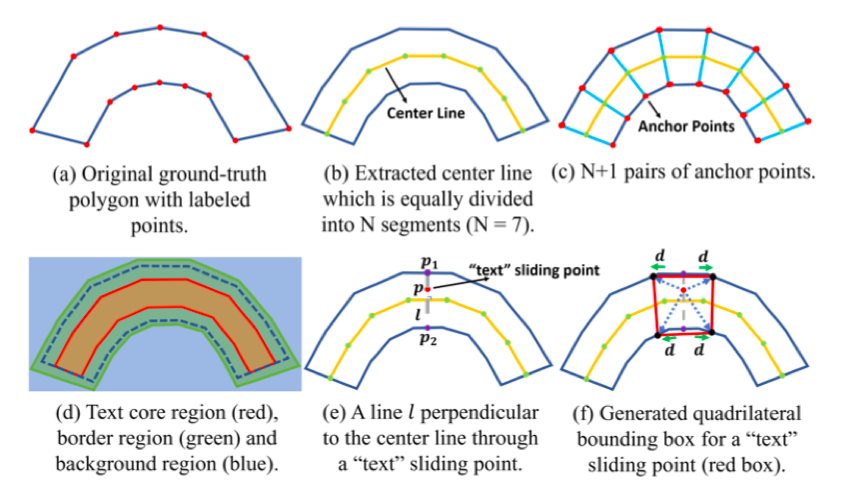
\includegraphics[width=.8\textwidth]{figure/detection/relatext_gt.png} 
    \caption{RelaText Label制作过程。} 
    \label{relatext_gt} 
\end{figure}

在构建graph时,基本原则为:同一graph的组件只来自于FPN中的同一层,并且这些组件的空间位置相近。具体地:
文本组件在graph中表现为一个节点,某一graph的节点的相邻节点来自于该节点的K近邻(两个文本组件的距离定义为
组件中心的空间距离)。所有的graph构建完成后,通过预测graph中的边的分类结果来确定组件是否属于同一文本。
边分类如图\ref{relatext_graph}所示:每条边的特征包括两个节点的视觉特征以及几何特征。几何特征定义为
[$\Delta(b_{i},b_{j})$,$\Delta(b_{i},b_{ij})$,$\Delta(b_{j},b_{ij})$],共18维度。其中$\Delta b_{i}$,
$\Delta b_{j}$,$\Delta b_{ij}$分别代表两组件的box以及两个box的并集。
$\Delta(b_{i},b_{j}) = (t_{x}^{ij},t_{y}^{ij},t_{w}^{ij},t_{h}^{ij},t_{x}^{ji},t_{y}^{ji})$定义如下:

$t_{x}^{ij} = (x^{i} - x^{j})/w^{i}$, $t_{y}^{ij} = (y^{i} - y^{j})/h^{i}$,

$t_{w}^{ij} = log(w^{i}/w^{j})$, $t_{h}^{ij} = log(h^{i}/h^{j})$,

$t_{x}^{ji} = (x^{j} - x^{i})/w^{j}$, $t_{y}^{ji} = (y^{j} - y^{i})/h^{j}$。




\begin{figure}[H]
    \centering
    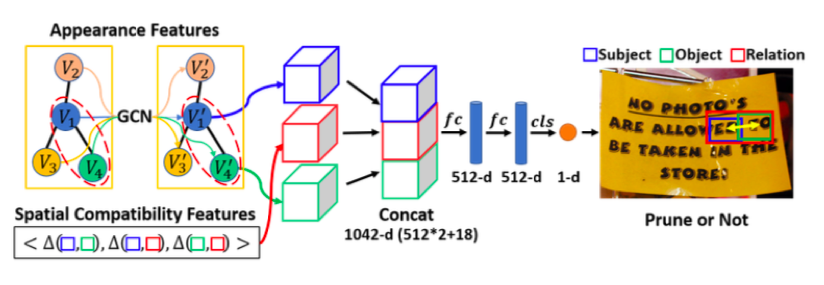
\includegraphics[width=.8\textwidth]{figure/detection/relatext_graph.png} 
    \caption{RelaText GCN中边分类过程。} 
    \label{relatext_graph} 
\end{figure}

\subsection{PuzzleNet}
PuzzleNet\cite{liu2020puzzlenet}属于bottom-up类型的任意形状文本检测器。通过GCN来连接各个文本组件。和ReLaText的不同在于graph的构建:
ReLaText是将同一尺度,K近邻的文本组件构建成一个graph,而PuzzleNet是一张图像内的所有组件构建一个graph。因为ReLaText中每个文本实例由大量的
文本组件构成(比较PuzzleNet和ReLaText网络生成文本组件),为了高效,所以一张图像需要构建多个graph单独处理。

\subsubsection{PuzzleNet的网络结构}
RelaText的网络结构如图\ref{puzzlenet_framework}所示,网络的backbone基于RRPN。首先预测出文本组件(旋转长方形),然后将nms后的所有文本组件构建一个graph(一张图像一个graph),
通过GCN网络来判断相邻节点是否连接。
\begin{figure}[H]
    \centering
    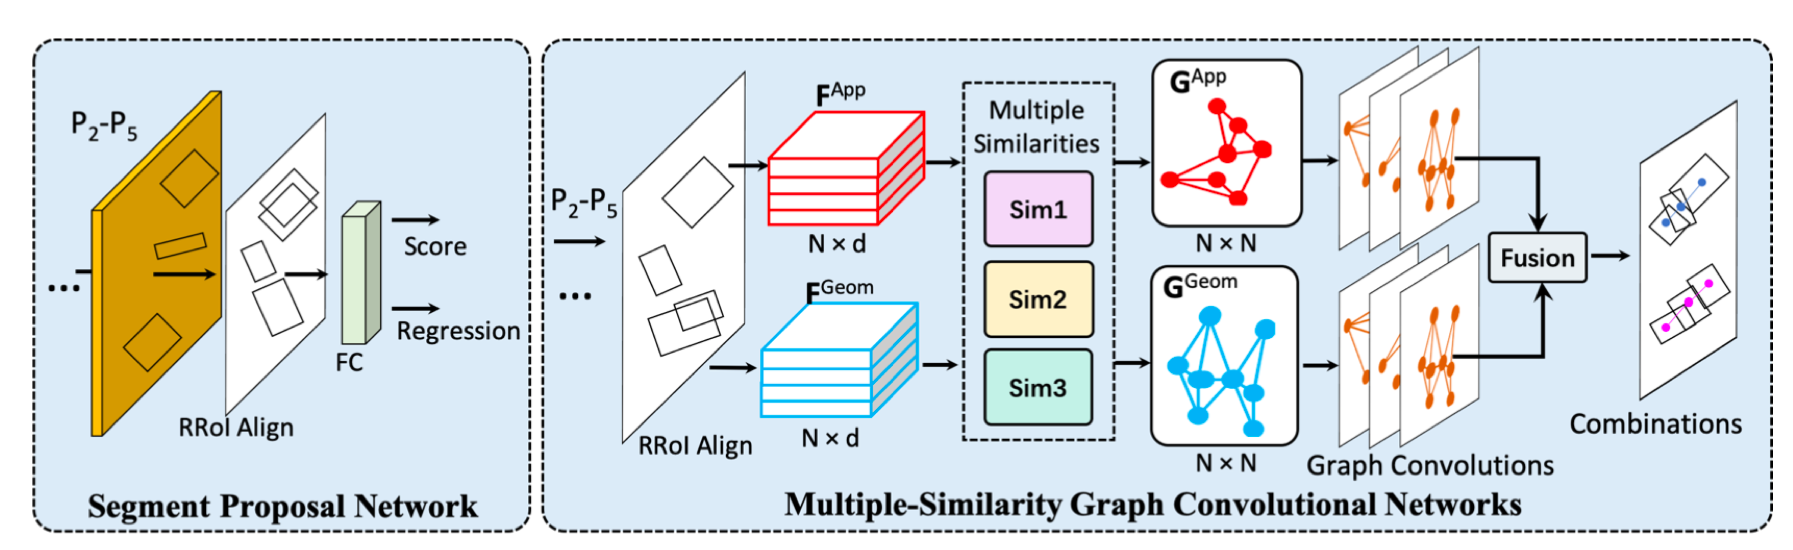
\includegraphics[width=.98\textwidth]{figure/detection/puzzlenet_framework.png} 
    \caption{PuzzleNet网络框架图。} 
    \label{puzzlenet_framework} 
\end{figure}

具体来说,网络的MSGCN模块中分为两个支路(appearance graph和geometry graph),其过程可用下式表达。

$link = classifier(cat(K(F_{App},F_{App})F_{App}W_{App} + F_{App}, K(F_{Geo},F_{Geo})F_{Geo}W_{Geo} + F_{Geo}))$,

其中,$F_{App}\in \Re^{Nxd}$代表视觉特征,$F_{Geo}\in \Re^{Nxd}$代表几何特征,$W\in \Re^{dxd}$,$K$代表相似性度量函数,$K(*)\in \Re^{NxN}$,$cat(*)\in \Re^{Nx2d}$。
相似性度量函数定义如下:

$K = \beta_{1}K_{1} + \beta_{2}K_{2} + \beta_{3}K_{3}, s.t. \beta_{1} + \beta_{2} + \beta_{3} = 1$,

$K_{1}(y_{1}, y_{2}) = \frac{y_{1}y_{2}^{T}}{|y_{1}||y_{2}|}$,
$K_{2}(y_{1}, y_{2}) = exp(-\frac{||y_{1} - y_{2}||^{2}}{2\sigma^{2}})$,
$K_{3}(y_{1}, y_{2}) = exp(-\frac{JSD(y_{1} , y_{2})}{2\sigma^{2}})$,$JSD$代表Jensen-Shannon Divergence。

可以看出$K(F_{App},F_{App})F_{App}W_{App} + F_{App}$和NonLocal模块的含义一致,起到特征加强的作用。

\begin{figure}[H]
    \centering
    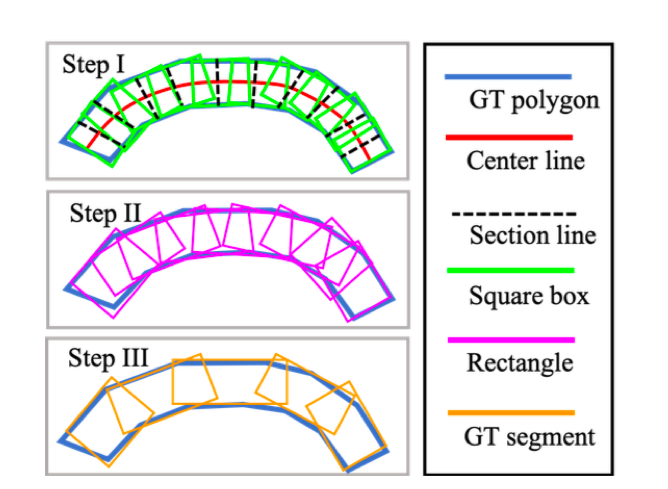
\includegraphics[width=.6\textwidth]{figure/detection/puzzlenet_gt.png} 
    \caption{PuzzleNet Label制作过程:1)生成大量的小的文本组件,2)相邻的小文本组件融合为长方形,3)将角度相近的长方形融合。} 
    \label{puzzlenet_gt} 
\end{figure}
% \subsubsection{PuzzleNet的后处理过程}
\subsection{DRRG (CVPR2020)}
DRRG\cite{zhang2020deep}属于bottom-up类型的任意形状文本检测器。将文本区域表示为多个文本组件,通过GCN来预测各个组件之间是否连接。
和ReLaText一样,一张图像的所有文本组件构建为多个graph,构建graph的算法和ReLaText不同。

\subsubsection{DRRG的网络结构}
DRRG的网络结构如图\ref{drrg_framework}所示:网络通过Text Compont Prediction模块来预测文本组件的属性(其backbone如图\ref{drrg_backbone}所示,文本组件生成过程如图\ref{drrg_gt}所示),
然后通过IPS\cite{wang2019linkage}算法构建多个Local Graphs,然后Relational Reasoning模块预测Local Graphs中边的连接关系,
最后融合Local Graphs的预测结果(一个文本实例的文本组件可能处于多个graph中),得到最后完整的文本组件的连接关系。
\begin{figure}[H]
    \centering
    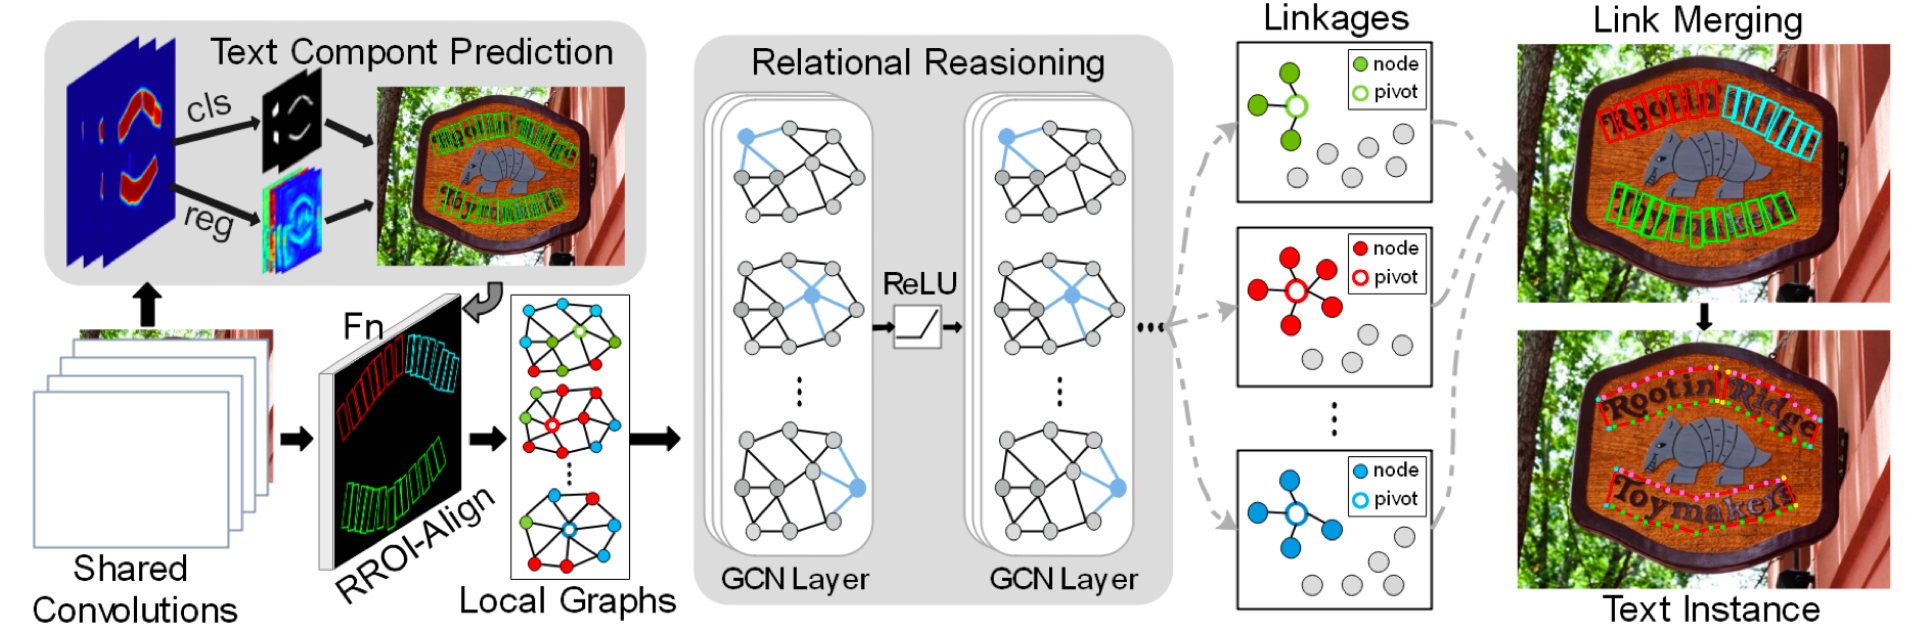
\includegraphics[width=.98\textwidth]{figure/detection/drrg_framework.png} 
    \caption{DRRG网络框架图。} 
    \label{drrg_framework} 
\end{figure}

Local Graphs的构建过程如下:1)选定pivot(按照文献\cite{wang2019linkage}的做法,依次将每个文本组件作为pivot);
2)以pivot为中心,2-hop(暂时理解为往外延伸2代节点,每个节点最多4个邻域,该理解需要进一步确认)的文本组件构建为一个graph;
寻找领域时的相似性度量如下所示:
$E_{s} = 1 - D(p, v_{i})/max(H_{m},W_{m}), v_{i} \in V_{p}$,$D(p, v_{i})$代表节点的文本组件中心的距离,$H_{m},W_{m}$
代表图像高宽。

\begin{figure}[H]
    \centering
    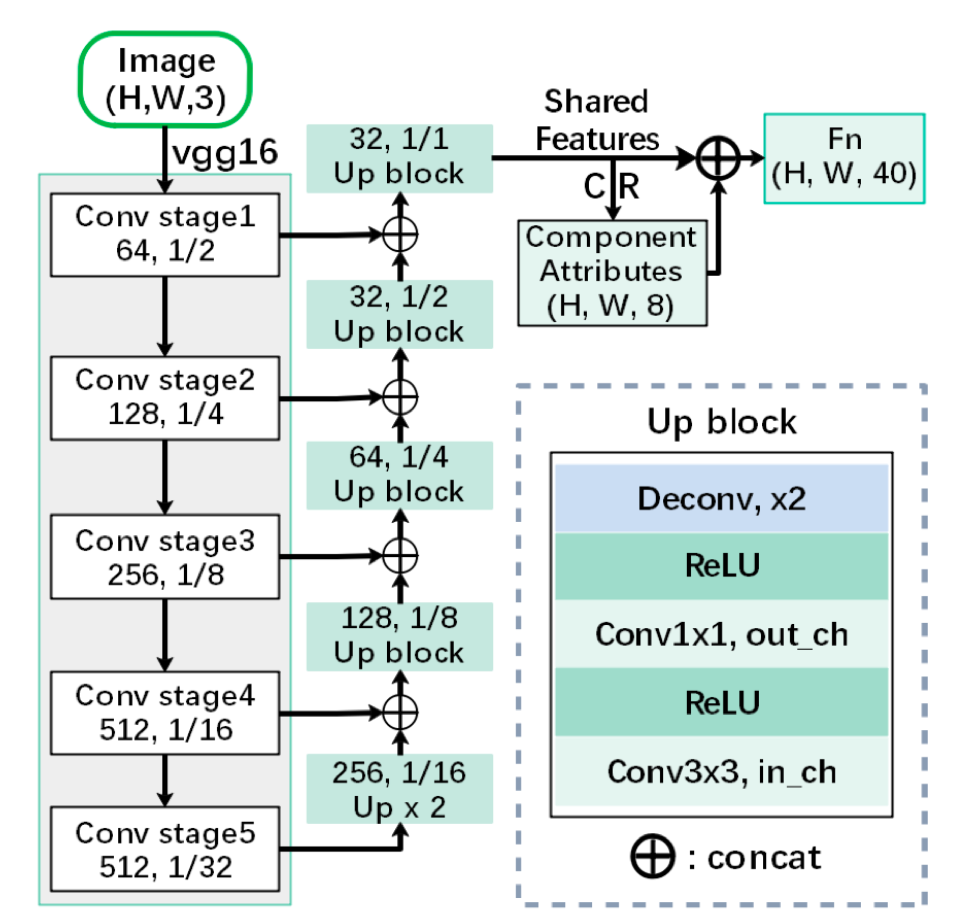
\includegraphics[width=.5\textwidth]{figure/detection/drrg_backbone.png} 
    \caption{DRRG的backbone。} 
    \label{drrg_backbone} 
\end{figure}

\begin{figure}[H]
    \centering
    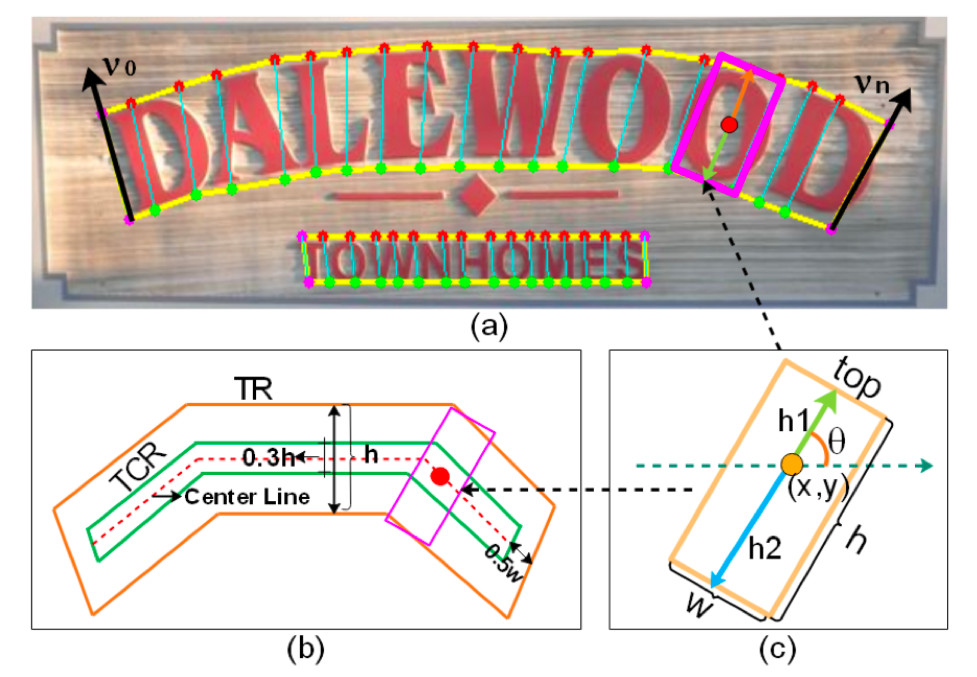
\includegraphics[width=.6\textwidth]{figure/detection/drrg_gt.png} 
    \caption{文本组件构建过程。} 
    \label{drrg_gt} 
\end{figure}

Local Graphs中节点特征以及连接矩阵如图\ref{drrg_graph}所示:节点特征由视觉特征$F_{r}$和几何特征构成$F_{g}$构成。
$F_{r}$由RRoI-Align进行提取,$F_{g}$由预测的几何向量($x,y,h,w,cos\theta,sin\theta$)经变换函数$\varepsilon$构成。

$\varepsilon_{2i} = cos(\frac{z}{1000^{2i/C_{\varepsilon}}}) , i \in (0, C_{\varepsilon}/2-1)$,

$\varepsilon_{2i+1} = sin(\frac{z}{1000^{2i/C_{\varepsilon}}}) , i \in (0, C_{\varepsilon}/2-1)$。

其中$C_{\varepsilon}$代表每个几何属性生成的Embedding向量的维度,最终几何特征$F_{g}$的维度为$6C_{\varepsilon}$。
\begin{figure}[H]
    \centering
    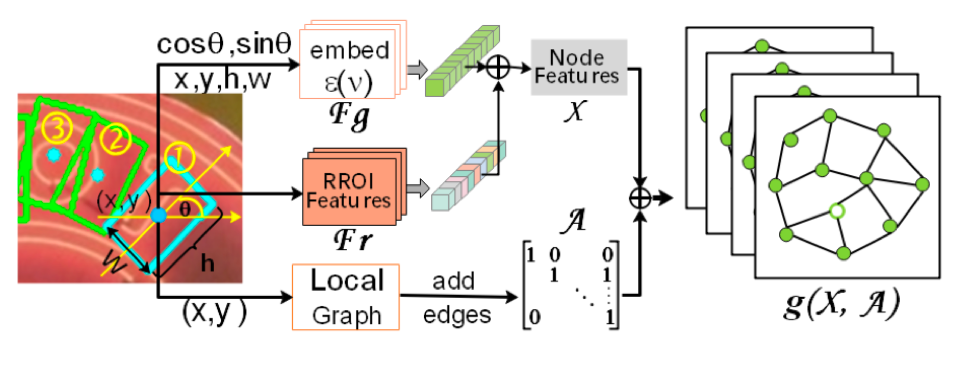
\includegraphics[width=.9\textwidth]{figure/detection/drrg_graph.png} 
    \caption{Graph中节点特征以及连接矩阵:节点特征由视觉特征和几何特征构成。} 
    \label{drrg_graph} 
\end{figure}
